% \iffalse
\let\negmedspace\undefined
\let\negthickspace\undefined
\documentclass[journal,12pt,twocolumn]{IEEEtran}
\usepackage{cite}
\usepackage{amsmath,amssymb,amsfonts,amsthm}
\usepackage{algorithmic}
\usepackage{graphicx}
\usepackage{textcomp}
\usepackage{xcolor}
\usepackage{txfonts}
\usepackage{listings}
\usepackage{enumitem}
\usepackage{mathtools}
\usepackage{float}
\usepackage{gensymb}
\usepackage{comment}
\usepackage{circuitikz}
\usepackage[breaklinks=true]{hyperref}
\usepackage{tkz-euclide} 
\usepackage{listings}
\usepackage{gvv}                                        
\def\inputGnumericTable{}                                 
\usepackage[latin1]{inputenc}                                
\usepackage{color}                                            
\usepackage{array}          
\usetikzlibrary{positioning, arrows.meta,shapes}
\usepackage{longtable}                                       
\usepackage{calc}                                             
\usepackage{multirow}                                         
\usepackage{hhline}                                           
\usepackage{ifthen}                                           
\usepackage{lscape}
\usepackage{amsmath}
\newtheorem{theorem}{Theorem}[section]
\newtheorem{problem}{Problem}
\newtheorem{proposition}{Proposition}[section]
\newtheorem{lemma}{Lemma}[section]
\newtheorem{corollary}[theorem]{Corollary}
\newtheorem{example}{Example}[section]
\newtheorem{definition}[problem]{Definition}
\newcommand{\BEQA}{\begin{eqnarray}}
\newcommand{\EEQA}{\end{eqnarray}}
\newcommand{\define}{\stackrel{\triangle}{=}}
\theoremstyle{remark}
\newtheorem{rem}{Remark}
\begin{document}

\bibliographystyle{IEEEtran}
\title{GATE-2021-BM-Q3}
\author{EE23BTECH11015 - DHANUSH V NAYAK$^{*}$% <-this % stops a space
}
\maketitle
\newpage
\bigskip
\renewcommand{\thefigure}{\arabic{figure}}
\renewcommand{\thetable}{\theenumi}
\textbf{Question:}Three resistive loads are connected to ideal voltage and current source as shown in circuit below. The voltage $V_{AB}$ across terminals A and B is equal to 
\begin{figure}[H] 
    \centering
    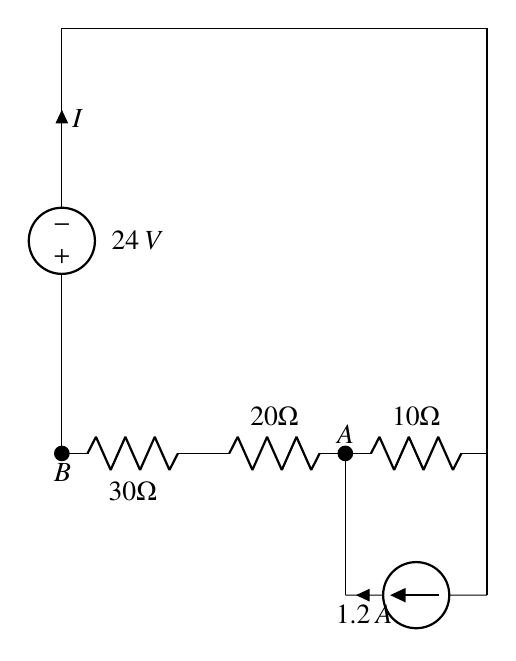
\begin{tikzpicture}[american, scale=0.9]

    \draw (2,0) to[R=$30\Omega$] (0,0) node[below] {$B$} node[circle,fill,inner sep=2pt]{};
    \draw (2,0) to[R=$20\Omega$] (4,0) node[above] {$A$} node[circle,fill,inner sep=2pt]{};
    \draw (4,0) to[R=$10\Omega$] (6,0) -- (6,6) -- (0,6);

    \draw (0,6) to [V=$24\,V$,i=$I$ ,invert] (0,0);

    \draw (4,0) -- (4,-2);
    \draw (6,-2) to[I, i=$1.2\,A$] (4,-2);
    \draw (6,-2) -- (6,0);
\end{tikzpicture}


    \caption{Circuit Diagram}
    \label{fig:gate_21_bm_q3_ckt}
\end{figure}
\hfill(GATE-2021-BM-Q3)\\
\solution 
\begin{table}[H]
\centering
\renewcommand\thetable{1}
\setlength{\extrarowheight}{9pt}
\resizebox{0.4\textwidth}{!}{
\begin{tabular}{|c|c|c|}
\hline
\textbf{Parameter} & \textbf{Description} \\ \hline
$I\brak{1}$ & Current only due to voltage source \\ \hline
$I\brak{2}$ & Current only due to current source\\ \hline
$I$ & Total Current by superposition \\ \hline
$V_{AB}$ &  Voltage across terminal A and B \\ \hline
$R_{eq}$ & Equivalent Resistance\\ \hline
\end{tabular}}
\caption{Parameter Table}
\label{tab:gate21_bm_Q3}
\end{table}

Using the superposition principle, First, consider the voltage source only:
\begin{figure}[H] 
    \centering
    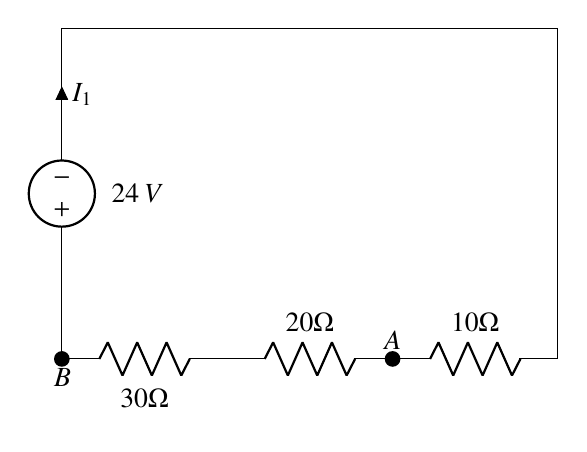
\begin{tikzpicture}[american, scale=0.7]
    % Draw resistors in series
    \draw (3,0) to[R=$30\Omega$] (0,0) node[below] {$B$} node[circle,fill,inner sep=2pt]{};
    \draw (3,0) to[R=$20\Omega$] (6,0) node[above] {$A$} node[circle,fill,inner sep=2pt]{};
    \draw (6,0) to[R=$10\Omega$] (9,0) -- (9,6) -- (0,6);

    % Draw battery
    \draw (0,6) to [V=$24\,V$,i=$I_{1}$ ,invert] (0,0);
\end{tikzpicture}
    \caption{Circuit considering only voltage source}
    \label{fig:gate_21_bm_q3_ckt_1}
\end{figure}
\begin{align}
    V &= I_{1}R_{eq}\\
    R_{eq} &= 30 + 20 + 10 = 60 \Omega\\
\end{align}
Therefore:
\begin{align}
    I_{1} &= -\frac{24}{60} \\
         &= -0.4 A\label{eq:gate21_Bm_q3_I1_result}
\end{align}
Now, considering current source only 
\begin{figure}[H] 
    \centering
 \begin{tikzpicture}[american, scale=1.4]
    % Draw resistors in series
    \draw (2,0) to[R=$30\Omega$,i=$I_2$] (0,0) node[below] {$B$} node[circle,fill,inner sep=2pt]{};
    \draw (2,0) to[R=$20\Omega$] (4,0) node[above] {$A$} node[circle,fill,inner sep=2pt]{};
    \draw (4,0) to[R=$10\Omega$] (6,0) -- (6,3) -- (0,3)--(0,0);
    \draw (4,0) -- (4,-2);
    \draw (6,-2) to[I, i=$1.2\,A$] (4,-2);
    \draw (6,-2) -- (6,0);
\end{tikzpicture}
    \caption{Circuit considering only current source}
    \label{fig:gate_21_bm_q3_ckt_2}
\end{figure}
Writing KVL around the loop:
\begin{align}
    30\brak{I_2} + 20\brak{I_2} + 10\brak{I_2-1.2} &=0\\
    60I_2 -12 &=0\\
    I_2&= 0.2 A \label{eq:gate21_bm_q3_I2_res}
\end{align}
     
By superposition :   
\begin{align}
    I &= I_1 + I_2 \label{eq:gate21_bm_q3_sup}
\end{align}
Using \eqref{eq:gate21_Bm_q3_I1_result} and \eqref{eq:gate21_bm_q3_I2_res} in \eqref{eq:gate21_bm_q3_sup}
\begin{align}
    I &= -0.2A    \label{eq:gate21_bm_q3_Ivalue}
\end{align}
Thus,
\begin{align}  
    V_{AB} &= 50\times I
\end{align}
From \eqref{eq:gate21_bm_q3_Ivalue}
\begin{align}
    V_{AB} &= -10 V \label{eq:gate_21_bm_finalans} 
\end{align}
\end{document}

